%! TeX program = xelatex

\documentclass[12pt, a4paper]{article}
\usepackage{cmap}
\usepackage[fontsize=12pt]{scrextend}
\usepackage[T2A]{fontenc}
\usepackage[utf8]{inputenc}
\usepackage[english,russian]{babel}
\usepackage{amsmath,amsfonts,amssymb,amsthm,mathtools}
\usepackage[left=20mm, top=20mm, right=20mm, bottom=20mm, nohead, footskip=1cm]{geometry}
\usepackage{multirow}
\usepackage{array}
\usepackage{multicol}
\usepackage{graphicx}
\usepackage{wrapfig}
\usepackage{indentfirst}
\usepackage{enumitem}

\usepackage{polyglossia}
\usepackage{titlesec}
\usepackage{sectsty}
\usepackage{setspace}
\usepackage{fontspec}
\defaultfontfeatures{Mapping=tex-text}

\usepackage{lipsum}
\usepackage{tocloft}
\usepackage[dvipsnames]{xcolor}

\usepackage{caption}
%\captionsetup{labelfont=it, textfont=it}
%\captionsetup[figure]{name=Схема}

\usepackage{hyperref}

\hypersetup{
    colorlinks=false,
    linktoc=all
}
\urlstyle{same}

\setmainlanguage{english}
\setotherlanguage{russian}
\setkeys{russian}{babelshorthands=true}
\setmainfont{Times New Roman}
\newfontfamily\cyrillicfont{Times New Roman}
\let\cyrillicfonttt\ttfamily
%\onehalfspacing

%\allsectionsfont{\centering}
\renewcommand{\cftsecleader}{\cftdotfill{\cftdotsep}}

%======================================SECTIONING=========================================
%\makeatletter
%\renewcommand*\l@section{\@dottedtocline{1}{1.5em}{2.3em}}
%\makeatother
%======================================SECTIONING=========================================

\pretolerance=6000
\tolerance=3000
\emergencystretch=4pt

\setlength\intextsep{10pt}

\graphicspath{{./visuals/}}
\setlength{\parskip}{0.3125cm}
\setlength{\parindent}{1.25cm}
\setlength{\columnsep}{1cm}
\author{Grigoryev Mikhail}
\title{Algs lab}

\begin{document}

\thispagestyle{empty}

\vspace{30mm}

\begin{center}
FEDERAL STATE AUTONOMOUS EDUCATIONAL INSTITUTION \\
OF HIGHER EDUCATION \\
ITMO UNIVERSITY

\vspace{40mm}

{\large \textbf{Report \\
on the practical task No. 1 \\
"Experimental time complexity analysis"}}
\end{center}

\vspace{15mm}

\begin{flushright}
{\large Performed by \\
\textit{Mikhail Grigoryev \\
Academic group J4133c \\}
Accepted by \\
Dr Petr Chunaev}
\end{flushright}

\vspace{100mm}

\begin{center}
St. Petersburg \\
2022
\end{center}

\newpage

\section*{Goal}
\addcontentsline{toc}{section}{Goal}

Experimental study of the time complexity of different algorithms.

\section*{Formulation of the problem}
\addcontentsline{toc}{section}{Formulation of the problem}

For each $n$ in range [1, 2000] the average computer execution time of programs implementing the algorithms and functions below (for five runs) is to be measured using timestamps. The obtained data is to be plotted showing the average execution time as a function of $n$. Theoretical time complexities are to be calculated and compared to empyrical.

\begin{enumerate}
\item Generate a random vector $v = [v_1, v_2, \cdots, v_n]$ with non-negative elements. For $v$, implement:
	\begin{itemize}
	\item $f(v) = const$;
	\item $f(v) = \sum_{k=1}^n v_k$;
	\item $f(v) = \prod_{k=1}^n v_k$;
	\item supposing the elements of $v$ are the coefficients of a polynomial $P$ of degree $n-1$, calculate the value $P(1.5)$ by a direct calculation of $P(x) = \sum_{k=1}^n v_k x^{k-1}$ and by Horner's method by representing the polynomial as:
		\[ P(x) = v_1 + x(v_2 + x(v_3 + \cdots)) \]
	\item Bubble Sort of the elements of $v$;
	\item Quick Sort of the elements of $v$;
	\item Timsort of the elements of $v$.
	\end{itemize}
\item Generate random matrices $A$ and $B$ of size $n\times n$ with non-negative elements. Find the usual matrix product for $A$ and $B$.
\item Describe the data structures and design techniques used within the algorithms.
\end{enumerate}

\section*{Brief theoretical part}
\addcontentsline{toc}{section}{Brief theoretical part}

Time complexity of an algorithm on a dataset of size $n$ refers to the amount of time that a certain computer requires to execute the algorithm on that dataset. As computers have vastly different computing powers, time complexity is usually represented in the "big O" notation.

Definition:
\[ f(n) = O(g(n)) \quad\Leftrightarrow\quad \exists n_0, c>0: \quad \forall n>n_0 \quad 0 \leq f(n) \leq cg(n) \]
This represents that $f(N)$ grows no faster than $g(N)$, starting with datasets of size $N_0$.

Algorithms and functions implemented in this task are:
\begin{itemize}
	\item Constant function (implementation is trivial). Time complexity is $O(1)$ as there are no calculations which depend on the size of the input dataset.
	\item Sum function is taken from python3 numpy library. Time complexity is $O(n)$, as to add all items within a vector, we must iterate over all of them.
	\item Product function is also taken from numpy library. Time complexity is again $O(n)$ due to iteration over all items within the random input vector.
	\item Direct polynomial evaluation was implemented trivially, as we needed to calculate each term individually. For $x^{k-1}$ numpy power function was used. Time complexity of numpy.power is $O(1)$ so total complexity of the computation is proportional to the number of terms, or $O(n)$.
	\item Horner method of polynomial evaluation was implemented via a recursive function. Time complexity is still $O(n)$, as the number of recursive function calls is equal to $n$ and all of them are executed at a constant rate.
	\item Bubble sort algorithm was faster to write by hand than to find an implementation of as it is rarely used due to its inefficiency. Time complexity is $O(n^2)$, as in worst case scenario (reversed order) for every item in the random input vector we will have to iterate over every other item. Average time of bubble sort can vary vastly, as it works fine with inputs close to being sorted.
	\item Quicksort algorithm was taken from numpy library. Time complexity of quicksort depends on how the pivot point is selected. Generally, it has complexity of $O(n \log n)$.
	\item Timsort is python's default sorting algorithm in its standard library, so standard library was used. It finds ordered runs within the input vector and utilizes them to sort the vector faster (with a combination of merge and insertion sorting algorithms). It has time complexity of $O(n \log n)$ as it is impossible to sort a vector faster than $O(n \log n)$ (unless the vector consists only of numerical values, then sorting can be done in linear time).
	\item Trivial implementation of matrix multiplication without any optimization proved to calculate the matrix product of $A$ and $B$ very slowly. Thus, numpy library function matmul uses optimized BLAS (Basic Linear Algebra Subprograms) method. It has time complexity of $O(n^3)$ but supposedly low constants, so computations don't take years.
\end{itemize}

For convenience, random input vector (and matrices) was generated once per all 2000 measurements and smaller datasets were created by slicing the initial random vector. E.g. if $n=420$, random vector for this computation will be \textit{v[:420]} and random matrix will be \textit{A[:420, :420]}.

For random input vector and random input matrices numpy arrays (dynamic arrays, essentially) were used.

\newpage

\section*{Results}
\addcontentsline{toc}{section}{Results}

Measurements of average execution time of constant function with time complexity $O(n)$ showed that constant time is needed in order to return a constant.
\begin{figure}[!h]
\centering
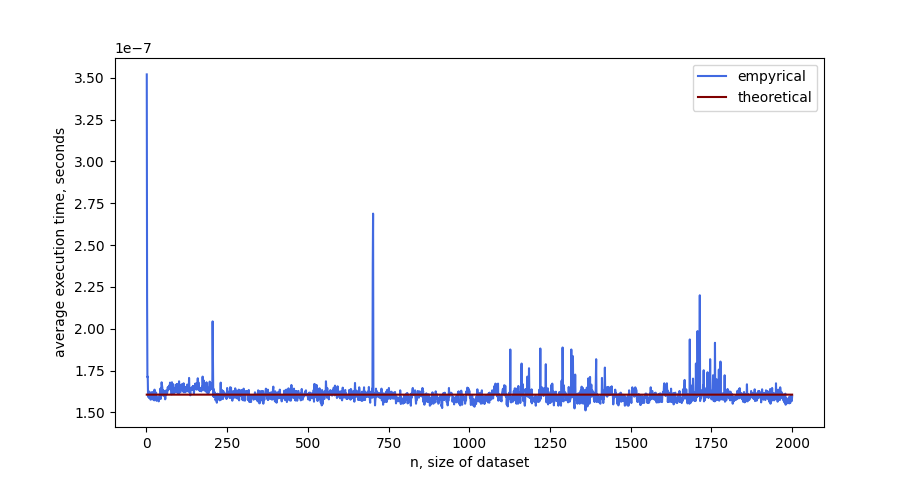
\includegraphics[width=0.9\textwidth]{const.png}
\caption{Empyrical and theoretical time complexities of an algorithm implementing the function $f(v)=1$.}
\end{figure}
Deviations from the constant are minimal and can be caused by system processes interrupting the program, as it is utilizing only one processor core.

Summation of all items within a random vector indeed was executed in linear time, as shown in the graph below.
\begin{figure}[!h]
\centering
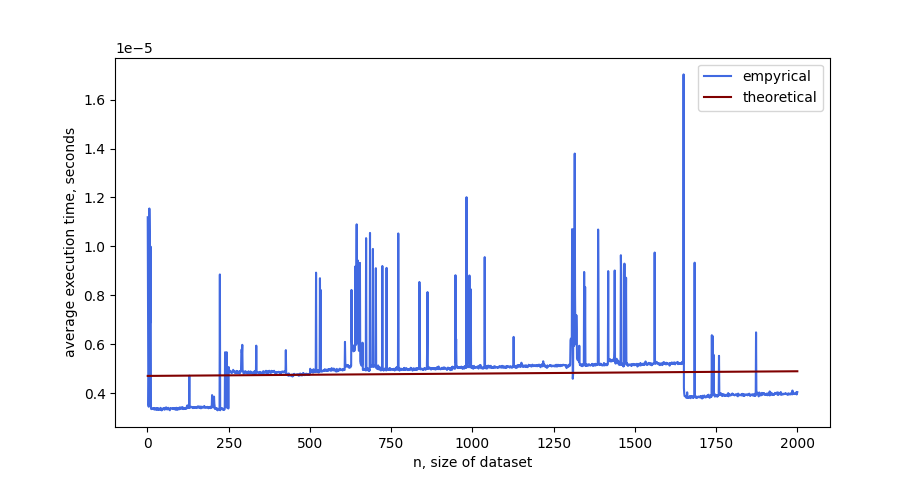
\includegraphics[width=0.9\textwidth]{sum.png}
\caption{Empyrical and theoretical time complexities of an algorithm implementing the function $f(v)=\sum_{k=1}^{n} v_k$.}
\end{figure}
The computation was done in linear time, although the slope of the line seems low. This can be caused by simple mathematical operators such as "+" to be processed really fast.

Similar trends were observed with the product function. The slope, however, is higher as "*" operator is processed slower than "+". Several slopes can be calculated because of system interferences.
\begin{figure}[!h]
\centering
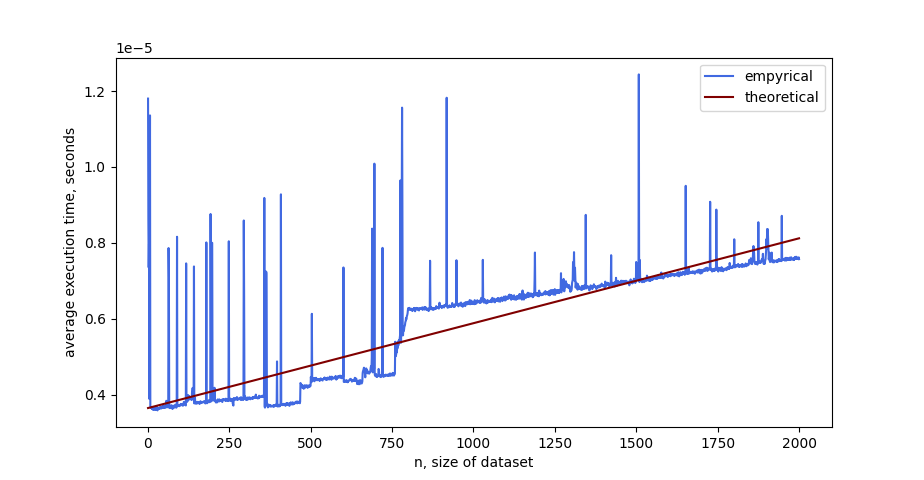
\includegraphics[width=0.9\textwidth]{prod.png}
\caption{Empyrical and theoretical time complexities of an algorithm implementing the function $f(v)=\prod_{k=1}^{n} v_k$.}
\end{figure}

Polynomial evaluation takes more time than the former algorithms, so random system interferences do not impact the measurements as much. Clear linear trend can be observed in direct polynomial evaluation.
\begin{figure}[!h]
\centering
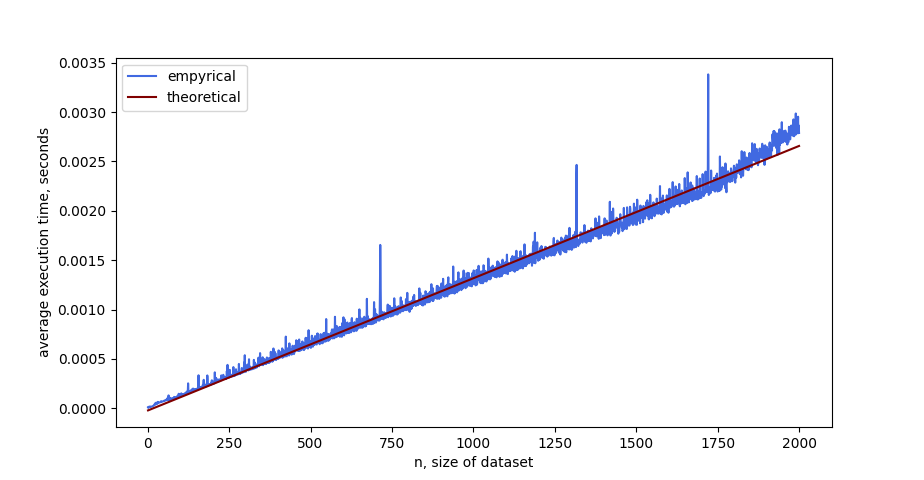
\includegraphics[width=0.9\textwidth]{polydirect.png}
\caption{Empyrical and theoretical time complexities of an algorithm implementing direct term-by-term evaluation of a polynomial.}
\end{figure}

\newpage

Horner's method of evaluation of a polynomial at a certain point gave similar results with a linear trend.
\begin{figure}[!h]
\centering
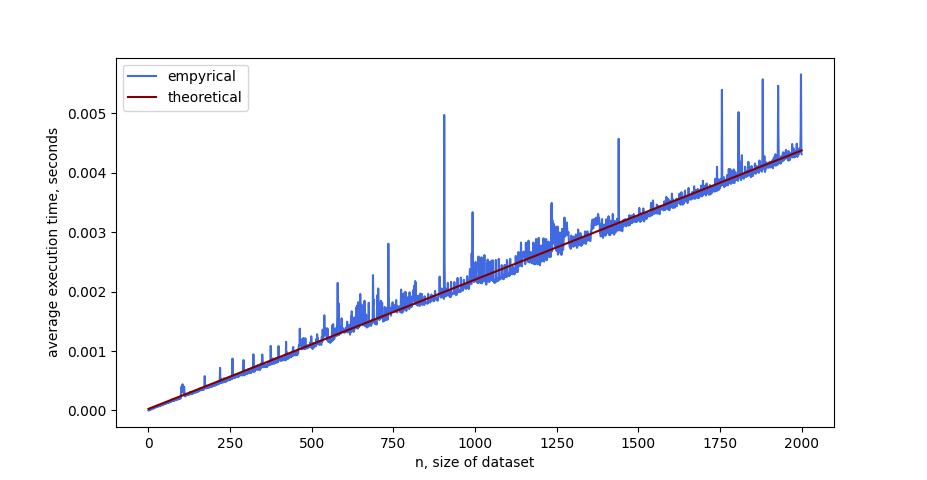
\includegraphics[width=0.9\textwidth]{polyhorner.png}
\caption{Empyrical and theoretical time complexities of an algorithm implementing Horner's method of evaluation of a polynomial.}
\end{figure}

A vastly different picture was observed with bubble sort. It gave a generally parabolic trend, however the deviation of execution time grew as datasets increased in size. This could be caused by bubble sorting algorithm being really dependent on the starting condition of the input vector.
\begin{figure}[!h]
\centering
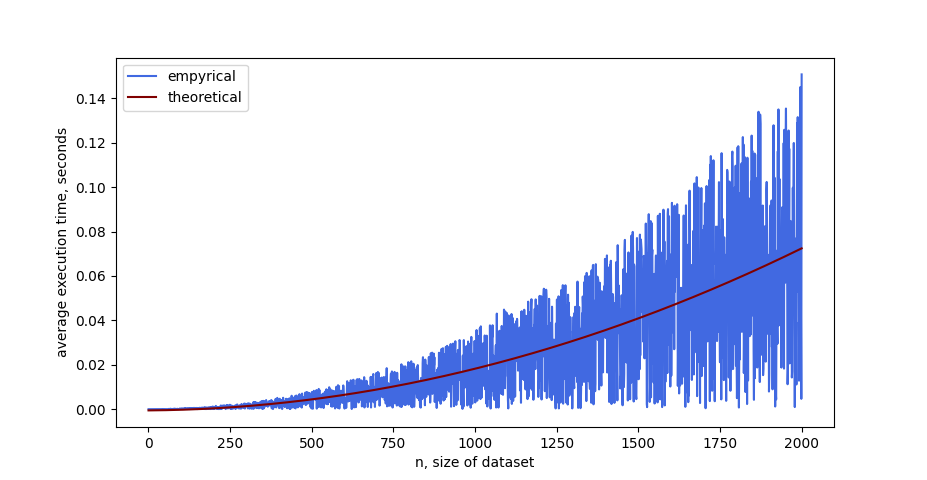
\includegraphics[width=0.9\textwidth]{bubblesort.png}
\caption{Empyrical and theoretical time complexities of a bubble sorting algorithm.}
\end{figure}

Clear $O(n \log n)$ time complexity can be observed in the graph below, where execution time of quicksort algorithm is depicted.
\begin{figure}[!h]
\centering
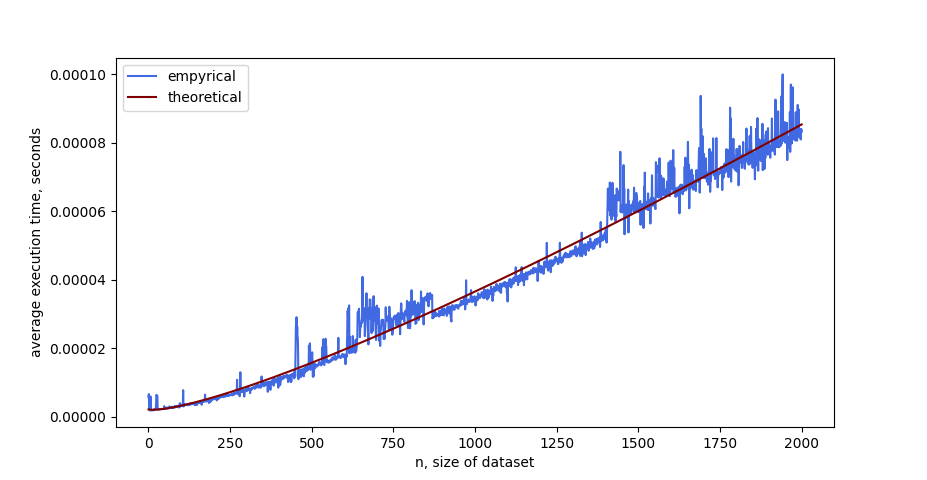
\includegraphics[width=\textwidth]{quicksort.png}
\caption{Empyrical and theoretical time complexities of a quicksort algorithm.}
\end{figure}
Deviation is minimal and seems caused by system interruptions as the deviation incresed and decreased in a step manner.

\newpage

Timsort gave an $n \log n$ tendency, although visually it resembles linear time. Thus it can be stated, that timsort is significantly more time efficient than quicksort.
\begin{figure}[!h]
\centering
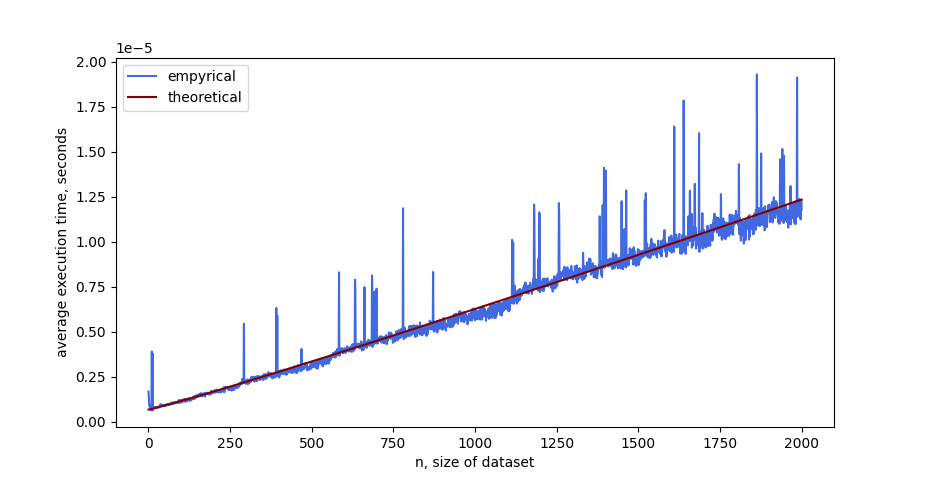
\includegraphics[width=\textwidth]{timsort.png}
\caption{Empyrical and theoretical time complexities of a timsort algorithm.}
\end{figure}

Matrix multiplication is a time consuming task which usually has time complexity of $O(n^3)$. Constants decide, whether computations will take seconds or hours, in that case. As shown in the graph below, cubic time was measured for numpy matmul implementation of matrix multiplication.
\begin{figure}[!h]
\centering
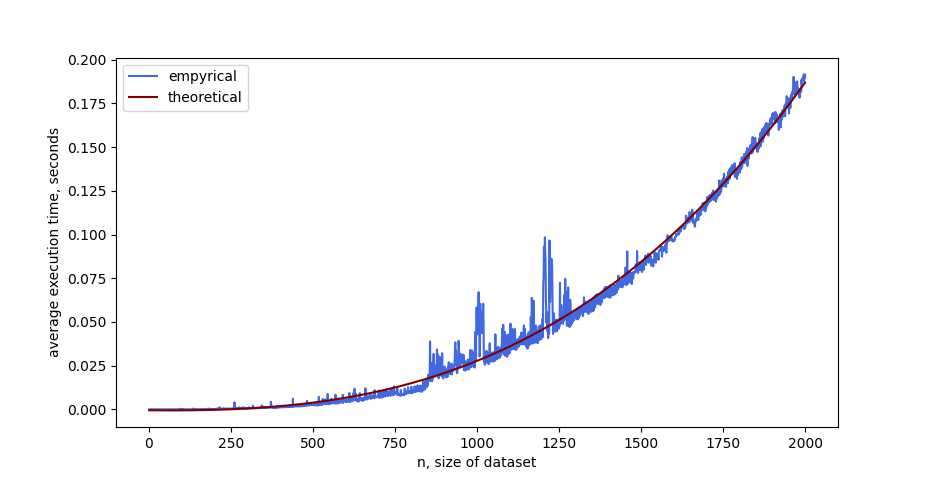
\includegraphics[width=0.9\textwidth]{matmul.png}
\caption{Empyrical and theoretical time complexities of an algorithm implementing matrix multiplication.}
\end{figure}

\section*{Conclusions}
\addcontentsline{toc}{section}{Conclusions}

In this practical work average execution times of different algorithms and functions were measures. The results proved to correspond to theoretical time complexities. Deviations in execution times were supposedly caused by system processes interfering with the program running on one processor core.

\section*{Appendix}
\addcontentsline{toc}{section}{Appendix}

GitHub link: \url{https://github.com/Dormant512/itmo_lab_listings/blob/main/lab1.py}.

\begin{figure}[!h]
\centering

\includegraphics[width=0.3\textwidth]{qr_lab1.png}
\end{figure}


\end{document}
